% Created 2021-09-11 Sat 16:41
% Intended LaTeX compiler: xelatex
\documentclass[letterpaper]{article}
\usepackage{graphicx}
\usepackage{grffile}
\usepackage{longtable}
\usepackage{wrapfig}
\usepackage{rotating}
\usepackage[normalem]{ulem}
\usepackage{amsmath}
\usepackage{textcomp}
\usepackage{amssymb}
\usepackage{capt-of}
\usepackage{hyperref}
\usepackage[margin=1in]{geometry}
\usepackage{fontspec}
\usepackage{indentfirst}
\setmainfont[ItalicFont = LiberationSans-Italic, BoldFont = LiberationSans-Bold, BoldItalicFont = LiberationSans-BoldItalic]{LiberationSans}
\newfontfamily\NHLight[ItalicFont = LiberationSansNarrow-Italic, BoldFont       = LiberationSansNarrow-Bold, BoldItalicFont = LiberationSansNarrow-BoldItalic]{LiberationSansNarrow}
\newcommand\textrmlf[1]{{\NHLight#1}}
\newcommand\textitlf[1]{{\NHLight\itshape#1}}
\let\textbflf\textrm
\newcommand\textulf[1]{{\NHLight\bfseries#1}}
\newcommand\textuitlf[1]{{\NHLight\bfseries\itshape#1}}
\usepackage{fancyhdr}
\pagestyle{fancy}
\usepackage{titlesec}
\usepackage{titling}
\makeatletter
\lhead{\textbf{\@title}}
\makeatother
\rhead{\textrmlf{Compiled} \today}
\lfoot{\theauthor\ \textbullet \ \textbf{2021-2022}}
\cfoot{}
\rfoot{\textrmlf{Page} \thepage}
\titleformat{\section} {\Large} {\textrmlf{\thesection} {|}} {0.3em} {\textbf}
\titleformat{\subsection} {\large} {\textrmlf{\thesubsection} {|}} {0.2em} {\textbf}
\titleformat{\subsubsection} {\large} {\textrmlf{\thesubsubsection} {|}} {0.1em} {\textbf}
\setlength{\parskip}{0.45em}
\renewcommand\maketitle{}
\author{Houjun Liu}
\date{\today}
\title{Illustrating electric fields}
\hypersetup{
 pdfauthor={Houjun Liu},
 pdftitle={Illustrating electric fields},
 pdfkeywords={},
 pdfsubject={},
 pdfcreator={Emacs 27.2 (Org mode 9.4.4)}, 
 pdflang={English}}
\begin{document}

\maketitle
Yes, you could do this.

\begin{figure}[htbp]
\centering
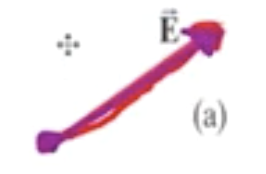
\includegraphics[width=.9\linewidth]{./Screen Shot 2020-08-24 at 8.54.03 PM.png}
\caption{Oooh! A \textbf{single} vector!}
\end{figure}

And theoretically draw infinite metric tonnes of these around an object.
But that's inefficient. We could instead think about electric fields as
infinitely expanding in lines that travel from the center of the object
outwards:

\begin{figure}[htbp]
\centering
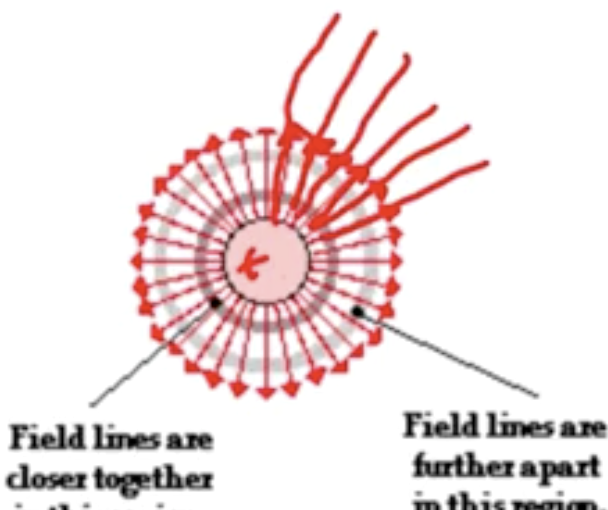
\includegraphics[width=.9\linewidth]{./Screen Shot 2020-08-24 at 8.57.21 PM.png}
\caption{Screen Shot 2020-08-24 at 8.57.21 PM.png}
\end{figure}

Well, here's a problem. This diagram does not show the magnitude of the
charge.

Well, fear not! Notice that there are shaded circles behind the red
arrows? The density of these circles dictate the magnitude of the charge
--- the denser the circles, the higher the magnitude.
\end{document}
